% Format teze zasnovan je na paketu memoir
% http://tug.ctan.org/macros/latex/contrib/memoir/memman.pdf ili
% http://texdoc.net/texmf-dist/doc/latex/memoir/memman.pdf
% 
% Prilikom zadavanja klase memoir, navedenim opcijama se podešava 
% veličina slova (12pt) i jednostrano štampanje (oneside).
% Ove parametre možete menjati samo ako pravite nezvanične verzije
% mastera za privatnu upotrebu (na primer, u b5 varijanti ima smisla 
% smanjiti 
\documentclass[12pt,oneside]{memoir}
\newcommand\tab[1][0.5cm]{\hspace*{#1}} 
% Paket koji definiše sve specifičnosti master rada Matematičkog fakulteta
\usepackage[latinica,biblatex]{matfmaster} 
\usepackage{verbatim}
\usepackage{url}
\usepackage{hyperref}
\newtheorem{primer}{Primer}

\usepackage[latinica]{pangrami}
\usepackage{listings}
\usepackage{color}
 
\definecolor{codegreen}{rgb}{0.6,0,0}
\definecolor{codegray}{rgb}{0.5,0.5,0.5}
\definecolor{codepurple}{rgb}{0.169, 0.169, 0.169}
\definecolor{backcolour}{rgb}{0.95,0.95,0.92}
 
\lstdefinestyle{mystyle}{
    backgroundcolor=\color{backcolour},   
    commentstyle=\color{codegreen},
    keywordstyle=\color{codegreen},
    numberstyle=\tiny\color{codegray},
    stringstyle=\color{codepurple},
    basicstyle=\footnotesize,
    breakatwhitespace=false,         
    breaklines=true,                 
    captionpos=b,                    
    keepspaces=true,                 
    numbers=left,                    
    numbersep=5pt,                  
    showspaces=false,                
    showstringspaces=false,
    showtabs=false,                  
    tabsize=2
}
 
\lstset{style=mystyle}




% Datoteka sa literaturom u BibTex tj. BibLaTeX/Biber formatu
\bib{literatura}

% Ime kandidata na srpskom jeziku (u odabranom pismu)
\autor{Ana Đorđević}
% Naslov teze na srpskom jeziku (u odabranom pismu)
\naslov{Automatsko generisanje test primera uz pomoć statičke analize i rešavača Z3}
% Godina u kojoj je teza predana komisiji
\godina{2017}
% Ime i afilijacija mentora (u odabranom pismu)
\mentor{dr Milena \textsc{Vujošević Janičić}, docent\\ Univerzitet u Beogradu, Matematički fakultet}
% Ime i afilijacija prvog člana komisije (u odabranom pismu)
\komisijaA{dr Filip \textsc{Marić}, vanredni profesor\\ Univerzitet u Beogradu, Matematički fakultet}
% Ime i afilijacija drugog člana komisije (u odabranom pismu)
\komisijaB{dr Milan \textsc{Banković}, docent \\ Univerzitet u Beogradu, Matematički fakultet}
% Ime i afilijacija trećeg člana komisije (opciono)
% \komisijaC{}
% Ime i afilijacija četvrtog člana komisije (opciono)
% \komisijaD{}
% Datum odbrane (odkomentarisati narednu liniju i upisati datum odbrane ako je poznat)
% \datumodbrane{}

% Apstrakt na srpskom jeziku (u odabranom pismu)
\apstr{%
}

% Ključne reči na srpskom jeziku (u odabranom pismu)
\kljucnereci{verifikacija softvera, testiranje softvera, SMT rešavači, Z3 rešavač, automatsko pronalaženje grešaka u programu, računarstvo}
\begin{document}
% ==============================================================================
% Uvodni deo teze
\frontmatter
% ==============================================================================
% Naslovna strana
\naslovna
% Strana sa podacima o mentoru i članovima komisije
\komisija
% Strana sa posvetom (u odabranom pismu)
\posveta{Mami i tati}
% Strana sa podacima o disertaciji na srpskom jeziku
\apstrakt
% Sadržaj teze
\tableofcontents*

% ==============================================================================
% Glavni deo teze
\mainmatter
% ==============================================================================

% ------------------------------------------------------------------------------
\chapter{Uvod}
% ------------------------------------------------------------------------------


% ------------------------------------------------------------------------------
\chapter{Testiranje}

Testiranje predstavlja važan deo životnog ciklusa razvoja softvera. 
Softver se implementira prema zahtevima korisnika sa ciljem rešavanja realnog problema ili kreiranja potrebne funkcionalnosti. Nakon implementacije, softver može u manjoj ili većoj meri odgovarati zahtevima. Svako ponašanje softvera koje se ne slaže sa zahtevima predstavlja grešku koju je potrebno detektovati i eliminisati. Testiranje predstavlja proveru da li je softver u potpunosti implementiran u skladu sa korisničkim zahtevima. Pored proveravanja samog softvera, testiranje uključuje proveravanje svih pratećih komponenti i karakteristika. Takođe, testiranje predstavlja jedan od načina specifikacije problema.
\par
Kako i najmanji problem može uništiti uloženi trud, u slučaju obimnih projekata nikada nije dovoljno testiranja. Sa porastom složenosti projekta, raste i značaj testiranja i provera celokupnog softverskog sistema kako bi se izbegli ishodi koji mogu da unište ceo projekat. 
S obzirom da se greške ne mogu izbeći, potrebno ih je što je moguće ranije otkriti kako bi njihovo otklanjanje bilo brže i jeftinije. Zbog prednosti koje se ostvaruju, najzastupljenije i trenutno najpopularnije metodologije razvoja softvera promovišu paralelnu implementaciju i pisanje testova za svaku od celina koja se razvija u okviru softverskog sistema. Pre isporučivanja softvera, neophodno je da uspešno prođu testovi za svaku od celina sistema.
\par 
U ovoj glavi opisan je proces testiranja po fazama u delu \ref{broj1}. U delu \ref{broj2} opisane su vrste testiranja softverskog sistema. U delu \ref{broj3} opisane su strategije testiranja. Načini izvršavanja testova opisani su u delu \ref{broj4}. Načini generisanja testova opisani su u delu \ref{broj5}. U ovom delu pored načina generisanja testova, navode se i primeri automatskog generisanja test primera. POPRAVITI
\section{Testiranje u procesu razvoja softvera} \label{broj1}
\par 
Testiranje softvera se u opštem slučaju sastoji od četiri faze pri čemu svaka faza obuhvata veliki broj aktivnosti. Proces testiranja sastoji se od faza planiranja, dizajniranja, izvršavanja i evaluacije testova.
\par
Planiranje predstavlja pripremu za ceo proces testiranja i uključuje definisanje zadataka koje je potrebno sprovesti kao i način njihovog izvršavanja. Tokom ove faze, definišu se vrste testova koje će biti sprovedene, metode testiranja, strategije kao i kriterijum završetka. Rezultat planiranja predstavlja skup dokumenata koji sadrže opštiji pogled na sistem koji će se testirati, aktivnosti koje će biti izvršene kao i alate koji će biti korišćeni.
\par 
Tokom faze dizajniranja testova, vrši se detaljna specifikacija načina na koje će se aktivnosti predviđene planom izvršiti. Pored toga, kreiraju se i precizna uputstva kako će se vršiti testiranje sistema. Tokom ove faze, analizira se sistem koji će biti testiran. Rezultat faze dizajniranja je skup test slučajeva i test procedura koja će biti korišćene u fazi izvršavanja testova.
\par
Izvršavanje testova se vrši radi provere funkcionalnosti sistema.
To je proces konkretne primene test slučajeva i test procedura formiranih na osnovu plana i dizajna. Izvršavanje testova obuhvata i dodatnu aktivnost praćenja statusa problema. Ova aktivnost podrazumeva eliminaciju prijavljenih problema kao i potvrđivanje da je problem rešen.
\par
Evaluacija testova predstavlja kreiranje izveštaja kojim se opisuje šta je testirano i potvrđivanje da je implementirani sistem spreman za korišćenje u skladu sa korisničkim zahtevima. Proces evaluacija uključuje i pregled rezultata dobijenih analizom izlaza test slučajeva.   

\section{Vrste testiranja} \label{broj2}

U literaturi se sreću različite podele testiranja softvera. Svaka je nastala kao posledica posmatranja različitih aspekata i pristupa provere softverskog sistema.
Jedan od pristupa odnosi se na testiranje različitih nivoa sistema. Nivoi testiranja mogu biti pojedinačni moduli, grupe modula (vezanih namenom, upotrebom, ponašanjem ili strukturom) ili ceo sistem.
U skladu sa pomenutom podelom, prema nivou testiranja, razlikujemo testove jedinice koda, testove prihvatljivosti, sistemske i istraživačke testove.
\par
Testiranjem jedinice koda (eng. \textit{Unit testing}) proverava se funkcionisanje delova sistema koji se nezavisno mogu testirati. U zavisnosti od konteksta i programske paradigme, to mogu se biti podprogrami ili veće komponente formirane od tesno povezanih jedinica. Ovom vrstom testiranja prolazi se svaki i najmanji deo sistema, pa upravo iz tog razloga ima važnu ulogu prilikom osiguravanja kvaliteta razvijenog softvera. Jedinični testovi definisani su standardom \textit{IEEE Standard for Software Unit Testing}. Cilj jediničnih testova je dokazivanje da komponenta ima predviđenu funkcionalnost. Ukoliko postoje greške u komponenti, one bi trebalo da budu otkrivene u fazi testiranja te komponente. Treba koristiti specijalne slučajeve ulaza, probati granice domena kao i nekorektan ulaz kako bi obezbedili da ne dolazi do pada softverskog sistema pri ovakvim situacijama.
\par
Testovi prihvatljivosti (eng. \textit{Acceptance testing}) 
treba da omoguće klijentima i korisnicima da se sami uvere da je napravljeni softver u skladu sa njihovim potrebama i očekivanjima.
Ovu vrstu testiranja izvode i procenjuju korisnici, a razvojni tim im pruža pomoć oko tehničkih pitanja, ukoliko za tim ima potrebe.
Klijent može da proceni sistem na tri načina: referentnim testiranjem, pilot testiranjem i paralelnim testiranjem. Kod referentnog testiranja, klijent generiše test slučajeve koji predstavljaju uobičajne uslove u kojima sistem treba da radi. Ove testove izvode korisnici kako bi procenili da li je softver implementiran u skladu sa očekivanjima. Pilot testiranje podrazumeva instalaciju sistema na privremenoj lokaciji i njegovu upotrebu. U ovom slučaju, testiranje se vrši simulacijom svakodnevnog rada na sistemu.
Paralelno testiranje se koristi tokom razvoja, kada jedna verzija softvera zamenjuje drugu ili kada novi sistem treba da zameni stari. 
Ideja je paralelno funkcionisanje oba sistema (starog i novog) čime se korisnici postepeno privikavaju i prelaze na korišćenje novog sistema.
\par 
Sistemsko testiranje (eng. \textit{System testing}) obuhvata proveravanje sistema kao celine. Ispituje se da li je ponašanje sistema u skladu sa specifikacijom zadatom od strane klijenta.
Ova vrsta testiranja stavlja naglasak na nefunkcionalne zahteve sistema kao što su brzina, efikasnost, otpornost na otkaze, uklapanje u okruženje u kojem će se sistem koristiti. 
Testiranje sistema obavlja se u drugačijim uslovima u odnosu na testiranje jedinica koda i testiranje prihvatljivosti. 
U proces testiranja sistema uključuje se ceo razvojni tim pod nadzorom rukovodioca projekta.
Testiranje sistema obuhvata nekoliko koraka pri čemu će u nastavku biti opisano testiranje performansi i instalaciono testiranje. 
\par
Tokom testiranja performansi, izvršavaju se testovi konfiguracije, kapaciteta, kompatibilnosti i bezbednosti kao i regresioni testovi. Testovima konfiguracije ispituje se ponašanje sistema u različitim hardverskim i softverskim okruženjima. 
Različite konfiguracije namenjene su različitim korisnicima sistema.
Ovim testovima proveravaju se sve konfiguracije sistema.
Testovima kapaciteta proverava se ponašanje sistema pri obradama velikih količina podataka. 
Proverava se i ponašanje sistema u slučaju kada skupovi podataka postignu svoje maksimalne kapacitete. 
Testovima kompatibilnosti proverava se način ostvarivanja komunikacije sistema sa drugim spoljnim sistemima.
Ovim testovima se proverava i da li je korisnički interfejs implementiran u skladu sa zahtevima klijenta. 
Svakako, pri testiranju važna karakteristika je bezbednost sistema.
Testovima bezbednosti proverava se da li su određene funkcionalnosti dostupne isključivo onim korisnicima kojima su namenjene. Proveravaju se i dostupnost, integritet i poverljivost svih skupova podataka. 
Regresiono testiranje podrazumeva primenu jednom napisanog test primera nekoliko puta za testiranje istog softvera. 
To se obično radi posle izmena u razvoju sistema, da bi se utvrdilo da nije došlo do lošeg rada nekih funkcija koje nisu bile obuhvaćene izmenama. 
Regresioni testovi garantuju da su performanse novog sistema barem jednake performansama starog. 

\par
Poslednja faza sistemskog testiranja je instalaciono testiranje.
Ova vrsta testiranja izvodi se instaliranjem softvera na klijentskoj mašini.
Prilikom instaliranja, sistem se konfiguriše u skladu sa okruženjem.
Ukoliko je potrebno, sistem se povezuje sa spoljnim uređajima i sa njima uspostavlja komunikaciju. 
Instalacioni testovi se izvršavaju u saradnji sa korisnicima. Ispituje se da li uslovi na klijentskoj mašini i okruženju negativno utiču na neke funkcionalne ili nefunkcionalne osobine sistema. 
Kada rezultati testiranja zadovoljavaju potrebe klijenta, testiranje se prekida i sistem se formalno isporučuje.
\par

Tokom istraživačkog testiranja (eng. \textit{Exploratory testing}) testeri pronalaze i proveravaju druge eventualne pravce korišćenja softverskog sistema. Na taj način podstiče se povećanje kreativnosti testera. Ova vrsta testiranja obuhvata aktivnosti prepoznavanja, kreiranja i izvršavanja novih test slučajeva. Istraživačko testiranje uglavnom ima smisla kada je aplikacija u svom finalnom obliku, kada tester može videti i druge alternativne pravce korišćenja sistema koji ranije nisu mogli biti predmet testiranja. Ukoliko se ova faza testiranja preskoči, postoji opasnost da neke funkcionalnosti sistema ne budu pokrivene testovima.
\par 
Opisani načini testiranja ilustrovani su piramidom testiranja na slici \ref{fig:piramida}. Piramidom testiranja ilustruje se redosled izvršavanja testova. Testiranje softvera počinje izvršavanjem testova jedinica koda, zatim slede testovi prihvatljivosti, sistemski i istraživački testovi. Najveći broj testova piše se za testiranje jedinica koda pri čemu svaki deo koda softverskog sistema mora biti pokriven bar jednim testom. Broj testova na svim nivoima zavisi od konkretnog projekta i prilagođava se potrebama klijenata.
\begin{figure}[!ht]
  \centering
  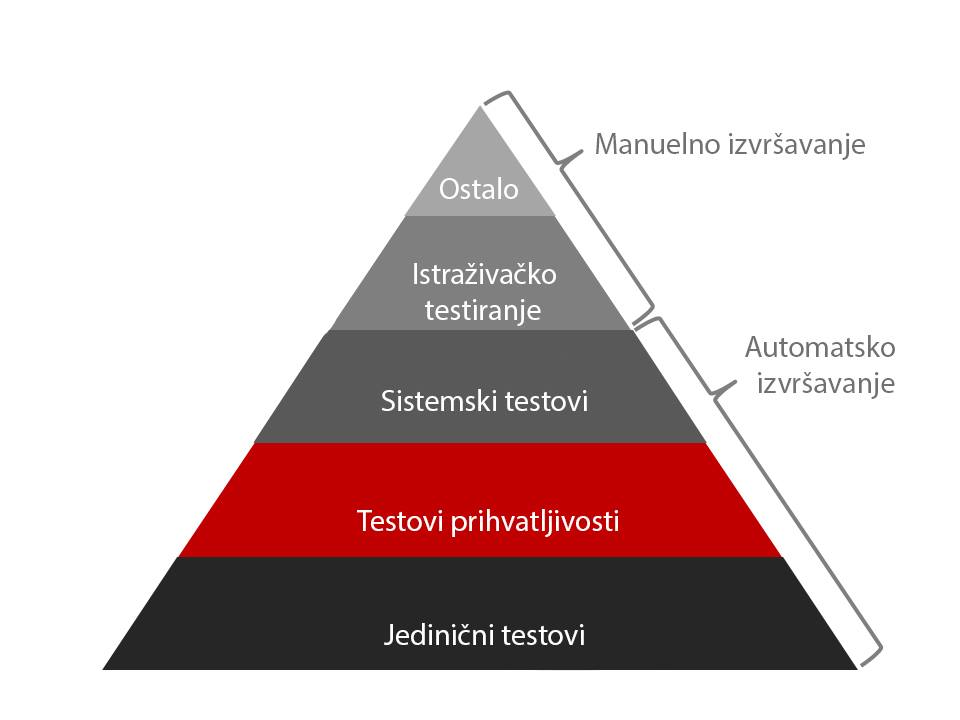
\includegraphics[width=0.9\textwidth]{piramida.jpg}
  \caption{Piramida testiranja softvera}
  \label{fig:piramida}
\end{figure}

Pored opisane podele i vrsta testova koji se izvršavaju, postoje i druge podele prema različitim kriterijumima testiranja. Više o podelama i podržanim načinima testiranja može se naći u literaturi \cite{TestingProcess}.

\section{Strategije testiranja} \label{broj3}
Testiranjem se obezbeđuje bolje razumevanje specifikacije problema, dizajna i implementacije rešenja. Pored otkrivanja grešaka, glavni ciljevi su obezbeđivanje traženog kvaliteta rešenja sistematskim testiranjem u kontrolisanim uslovima i identifikovanje potpunosti i korektnosti softvera. Tri najvažnije strategije za postizanje kvaliteta i detekciju grešaka su 
strategija crne kutije, strategija bele kutije i strategija sive kutije \cite{Strategies}.
 
\subsection{Strategija crne kutije}
Testiranje crnom kutijom (eng. \textit{Black Box Testing}) je strategija koja posmatra program kao zatvoreni sistem kako bi se uvrdilo ponašanje programa na
osnovu odgovarajućih ulaznih podataka. Ova strategija ne zahteva poznavanje strukture i analizu izvornog
koda, već samo osobine definisane specifikacijom softverskog sistema. Sprovodi se tako što se sistemu prosleđuju odgovarajući ulazni podaci a zatim se proverava da li je izlaz u skladu sa očekivanim. 
Ova strategija se između ostalog primenjuje prilikom testiranja web aplikacija ili servisa, gde se razmatra strana koju je generisao server na osnovu unetih podataka. Strategija testiranja crne kutije obično nije najbolji pristup, ali je uvek opcija. Prednost primene ove strategije je jednostavnost, pošto testiranje može biti vođeno bez poznavanja unutrašnje
strukture softverskog sistema. Ulazni podaci za testiranje sistema definišu se tako
da povećaju verovatnoću nalaženja greške i da smanje veličinu skupa testova. Ova strategija je potpuno fokusirana na funkcionalnosti rada aplikacije. \par
U nastavku će biti opisane dve metode koje primenjuju strategiju crne kutije. To su metoda klasa ekvivalencije i metoda graničnih vrednosti.
\par 
\subsubsection{Metoda klasa ekvivalencije}
Ideja metode deljenja na klase ekvivalencije (eng. \textit{Equivalence Partitioning}) je formiranje podskupova (klasa) podataka na osnovu ulaznih podataka. Jedna klasa sadrži ulazne podatke koji proizvode slične rezultate (izlazne vrednosti) pri testiranju. Na primer, jednu klasu podataka mogu činiti ulazni podaci koji otkrivaju istu grešku. U idealnom slučaju, podskupovi su međusobno disjunktni i ceo ulazni skup je pokriven. 
\par 
Da bismo identifikovali klase, posmatramo specifikaciju klijentskih uslova.
Za svaki uslov kreiramo po dve klase u zavisnosti da li je uslov ispunjen ili nije. Formiramo legalne klase koje obuhvataju ispravne i očekivane ulazne podatke kao i nelegalne klase koje obuhvataja sve ostale slučajeve ulaznih podataka.
\par 
Prednost metode deljenja na klase ekvivalencije je manji utrošak vremena pri testiranju softvera usled manjeg broja proverenih test slučajeva. Ulazne vrednosti u okviru jedne klase se smatraju ekvivalentnim, pa je za svaku klasu dovoljno pokretanje samo jednog test slučaja. Proveravanjem većeg broja test slučajeva u istoj klasi, ne identifikuju se nove greške u programu.

\subsubsection{Metoda graničnih vrednosti}
Kod metode graničnih  vrednosti (eng. \textit{Boundary Value  Analysis}) test slučajevi su
napravljeni  tako  da  reprezentuju  granice  odgovarajućih 
klasa (ulaznih podataka). Osnovu čini princip prethodno objašnjene 
metode klasa ekvivalencija.
Za svaki skup ulaznih podataka formiraju se tri klase, jedna validna i dve nevalidne. Validna klasa ima ispravne ulazne vrednosti, a nevalidne klase sadrže ulazne vrednosti koje ne pripadaju ispravnim opsezima. Vrednosti na granicama između validne i nevalidnih klasa nazivaju se test vektorima klasa.
Razlog  za korišćenje upravo ovih vrednosti za test vektore jesu česte softverske greške baš na
granicama opsega važenja. 

Za primenu ove metode, potrebno je više vremena za određivanje test slučajeve u poređenju sa drugim metodama strategije crne kutije zbog određivanja granica između validne i nevalidnih klasa.

\subsection{Strategija bele kutije}
Testiranje strategijom bele kutije (eng. \textit{White Box Testing}) zahteva pristup izvornom kodu, dobro poznavanje programskog jezika u kojem je sistem implementiran kao i dizajn konkrentog softverskog proizvoda. Plan testiranja izvodi se proučavanjem celokupnog programskog koda. Za svaku liniju koda može se proveriti da li se ona izvršava u zavisnosti od podataka na ulazu. Takođe, može se vršiti provera izvršavanja pojedinačnih funkcija. Specifičnim testovima proverava se postojanje beskonačnih petlji ili detektovanje delova koda koji se nikad ne izvrši. 
\par
Da bi se obezbedila primena strategije bele kutije, neophodno je i poznavanje interne logike i strukture koda kako bi se dizajnirali test slučajevi koji proveravaju kontrolne strukture programskog jezika. Kontrolne strukture obuhvataju naredbe grananja, uslovne naredbe, način menjanja tokova podataka i petlje.

Metode testiranja belom kutijom su testiranje grananja, testiranje osnovnih putanja, testiranje toka podataka i testiranje petlji.
Kod testiranja grananja testira se svaka moguća odluka u kontroli toka izvršavanja. Ova metoda uključuje i testiranje u slučaju spajanje odluka.  
Testiranje osnovnih putanja prati izvršavanje blokova naredbi i u zavisnosti od izvršenih delova koda formira test slučajeve za koje je potrebno pokrenuti softver. Kod testiranja toka podataka, formira se graf kontrole podataka koji sadrži informacije o pojavljivanju promenljivih u kodu i načinu njihovog menjanja. Kod testiranja petlji, proverava se ispravnost konstrukcija samih petlji.

Testiranje belom kutijom se primenjuje kod testova jedinica koda i sistemskih testova kako bi se eventualno pronašli delovi sistema koji proizvode neodgovarajuće ponašanje.
Nedostatak strategije bele kutije je visoka cena testiranja kao i zahtev za kvalifikovanim testerom. Pored toga,
mnoge putanje u sistemu mogu ostati netestirane pa se na taj način mogu sakriti potencijalne greške. 

\subsection{Strategija sive kutije}

Strategija testiranja sivom kutijom (eng. \textit{Gray Box Testing}) predstavlja kombinaciju prethodne dve strategije. Kod ove strategije postoji pristup nekom segmentu softvera, ali ne i kompletnom softverskom sistemu. Na osnovu analize poznatih delova koda koja odgovara testiranju bele kutije, formiraju se test slučajevi koji se zatim primenjuju na delove sistema o čijoj internoj strukturi nemamo informacija (odgovara testiranju crne kutije). Tehnika sive kutije koristi se u slučajevima testiranja integracije različitih delova koda. Ova strategija povećava pokrivenost koda test primerima kombinovanjem dve strategije. 
\par
Kada se primenjuje testiranje sivom kutijom, razlikujemo dve vrste testera. Prvu grupu čine kvalifikovani testeri koji na osnovu delimičnog pristupa izvornom kodu formiraju test slučajeve. Drugu grupu čine testeri čiji je zadatak samo izvršavanje dobijenih test slučajeva bez poznavanja interne strukture sistema. 
U zavisnosti od procenta celokupnog izvornog koda kome se može pristupiti, pokrivenost koda testovima može biti ograničena. 
\par
Metode testiranja sive kutije su ortogonalno testiranje, regresiono testiranje i testiranje obrazaca.
Ortogonalno testiranje koristi podskup svih kombinacija test slučajeva  dobijenih analizom dostupnih delova izvornog koda.
Regresioni testovi predstavljaju ponavljanje istih testova više puta u slučaju izmena pri razvoju sistema. Ovi testovi se sprovode kako bi se utvrdilo da promene u implementaciji nisu dovele do neželjenog ponašanja. 
Testiranje obrazaca podrazumeva primenu testova obrazaca pri dizajnu softverskih sistema
Ukoliko se sistem implementira prema nekom obrazcu projektovanja, testovima obrazaca proverava se da li je arhitektura sistema u skladu arhitekturom izabrarnog obrasca.

\section{Načini izvršavanja testova} \label{broj4}
U opštem slučaju, test se smatra uspešnim ukoliko je ponašanje sistema pri njegovom izvršavanju u skladu korisničkim zahtevima. Međutim, kod sve popularnije metodologije destruktivnog testiranja, test se smatra uspešnim ako se njegovim izvršavanjem otkriva postojanje greške u softveru.
\par
Izvršavanje testova sprovodi se na dva načina, automatizovano i manuelno. Manuelno  testiranje predstavlja ručno izvršavanje test slučajeva izabranim alatima. 
U većini slučajeva, tester prati niz koraka da bi verifikao neki segment softverskog sistema. Nakon toga, formira se izveštaj dobijenih rezultata.
\par
Automatizovano testiranje zahteva postojanje određenog koda koji je napisan da bi se automatizovali koraci pri izvršavanju test skripta. 
Datoteke koje sadrže logiku za testiranje nazivaju se test skripte i mogu biti pisane u svim programskim jezicima.

Automatsko testiranje se često koristi da bi se test slučajevi u okviru određenog test paketa koji su izvršeni manuleno mogu brzo izvršavati automatski. To je jako bitno kod regresionog testiranja s obzirom da 
regresiono testiranje sadrži sve test slučajeve koji su prethodno bili izvršeni nad sistemom ali I najnovije koji testiraju dodatu funkcionalnost.
Regression test često može uključivati I više hiljada test slučajeva tako da potreba za automatizacijom jasna. 
Motivi naravno su ušteda vremena a samim tim I novca.

Manuelno i automatizovano testiranje prate iste faze procesa testiranja
i mogu se primeniti na različitim novima i tipovima testiranja.
Manuelno i automatsko testiranje ima svoje prednosti i mane. U nastavku će biti navedene neke od njih. Automatizovano testiranje je brže, čime se ostvaruje velika ušteda vremena. Ušteda vremena je veoma značajna kod regresionih testova koji se često ponavljaju za velike sisteme. Automatizovano izvršavanje testova ne zahteva prisustvo testera pa je moguće njihovo stalno izvršavanje.
Automatizovano testiranje je sigurnije od manuelnog jer se kod manuelnog testiranja mogući propusti usled prekomernog rada ili umora testera. Prilikom testiranja, obično su na raspolaganju ograničeni resursi, čime se često onemogućuje efikasno izvršavanje manuelnog testiranja. Automatizovano testiranje je skuplje i zahteva obučeno osoblje. U slučaju čestog menjanja korisničkog interfejsa, manuelno testiranje je bolja opcija od automatizovanog. Svaka promena korisničkog interfejsa zahteva pisanje novih automatskih testova.


DFJDSF SDF SDF SDF SDFKDKKKKKKKKKKKKKKKKKKKKKKKKKKKKKKKKK
KKKKKKKKKKKKKKKKKKKKKKKKKKKKKKKKKKKKKKKKKKKKKKKKKKKKKKKKk
\section{Načini generisanja testova} \label{broj5}

AUTOMATSKO I MANUELNO 
Manuelno generisanje test primera podrazumeva da tester ručno piše testove za koje ce softver biti pokrenut. Ovakan način generisanja test primera može zahtevati veliki napor s obzirom da se vezuje za samu aplikaciju. Kod automatskog generisanja test primera korišćenjem drugih alata (programa) dobijaju se test primeri za koje se pokreće softver. 
Test primeri kod automatskog pristupa obično se vezuju za sam programski jezik u kojem je softver napisan. U ZAVISNOTI OD SLABOSTI JEZIKA

\subsection{Primeri automatskog generisanja test primera}
Rasplinuto testiranje (primer strategije crne kutije za generisanje test primera)
Fuzz testiranje je jedan od pristupa otkrivanja slabosti softvera zasno-
vano na tehnikama testiranja crne ili sive kutije. Definiše se kao analiza
graničnih vredosti gde se odreduje opseg dozvoljenih vrednosti konkretnog
ulaza i kreiraju se test vrednosti izvan granica. Fuzz testiranje se ne fo-
kusira samo na granične vrednosti već i na bilo koju ulaznu vrednost koja
može izazvati nedefinisano ili nebezbedno ponašanje. Može se definisati i kao metod otkrivanja grešaka softvera kreiranjem neočekivanih ulaza i
upravljanjem izuzecima. \par
Kako bi računalne aplikacije bile sigurne potrebno je testirati njihovu sigurnost. Jedna od metoda je nazvana testiranje Fuzz metodom. Tehniku je uspostavio Prof. Barton Miller sa sveučilišta u Wisconsinu 1988. kao studentski zadatak nazvan: “Operating System Utility Program 
Reliabilitiy –The Fuzz Generator“. Osnovna ideja testiranja Fuzz metodom jedavanje slučajnih ili pseudo-slučajnih podataka kao ulaz u testirani sustav. Ukoliko sustav prestane funkcionirati 
nakon nekog ulaza onda se taj niz podataka zabilježi za daljnju analizu. Danas se testiranje Fuzz 
metodom najviše koristi u velikim sustavima gdje se vrši testiranje na principu crne-kutije, zato 
što se pokazalo da Fuzz metoda daje jako dobar odnos cijene i vremena naspram kvalitete testiranja. Mogućnosti primjene su jako velike tako da se može testirati vrlo široki spektar različitih sustava od web-
aplikacija, protokola, funkcija u kodu i sl. 
\par
Za potrebe tes
tiranja stvaraju se fuzzing alati koji mogu biti različitih tipova i namijenjeni 
različitim 
profilima korisnika. Budući da je fuzzing alat efikasniji ukoliko je prilagođeniji 
testnom slučaju, neki
proizvođači prodaju biblioteke za razvoj fuzzing testova, n
o tada krajnji 
korisnici moraju sami implementirati konkretne testove što zahtjeva znanje i vrijeme. Prednost 
takvih testova što će su specijalizirani i samim time mogu podrobnije testirati sigurnosne 
propuste na testiranom objektu. Sa druge strane se nala
ze gotovi potpuni alati koji uz 
namještanje određeni parametara omogućuju korisniku da vrši testiranje. Prednost ovakvog 
pristupa je jednostavnost, dok mana je manje kvalitetno testiranje u odnosu na testove koji se 
rade specifično za objekt koji se testir
a.
Druga podjela alata se vrši na temelju toga da li mogu pamtiti stanje ili ne. Alati koje ne pamte 
stanje su statički i ne mogu simulirati protokol. Kompleksniji alati su bazirani na modelu 
komunikacije i mogu vršiti komunikaciju sa poslužiteljem te po p
otrebi varirati parametre 
komunikacije, mijenjati pakete u komunikaciji i sl. Fuzzing alati koji su bazirani na modelu su se 
pokazali puno boljim u pronalaženju sigurnosnih propusta. Ovakvi napredniji testovi mogu doći 
do dubljih pogrešaka u sustavu.
%METODE FUZZ TESTIRANJA \par
%Rasplinuto testiranje definise uopsteni pristup otkrivanja slabosti. Ako
%blize razmotrimo ovu metodologiju testiranja uoči ́cemo različite individu-
%alne metode koje se koriste za njenu primenu. Sledi pregled tih metoda.
%Random metoda
%Ova metoda je najmanje efikasna.  Podrazumeva ge-
%nerisanje slučajne vrednosti za testiranje nadaju ́ci se najboljem is-
%hodu.  Iznenađujuce je da su slabosti kriticnih delova softvera iden-
%tifikovani  upravo  ovom  metodom.   Može  biti  otežano  pronalazenje
%test primera koji je izazvao prekidanje programa u slučaju velikog
%broja slučajnih test vrednosti.
%Metoda izučavanja ulaznih vrednosti
%Razvoj test slučajeva počinje
%izučavanjem  svih  podržanih  struktura  podataka  i  prihvatljivih  op-
%sega vrednosti za svaki od njih.  Generišu se granični test uslovi na
%osnovu kojih se može proceniti preciznost ciljnog sistema.  Prednost
%je mogu ́cnost ponovne upotrebe test slučajeva na drugim implemen-
%tacijama koje koriste isti protokol ili format fajla.
%Rasplinuto testiranje grubom silom
%Rasplinuti  tester  započinje  testiranje ispravnim ulazom, a zatim u svakom %slede ́cem koraku menja  svaki  individualni  bajt  ili  karakter  niske  u  %zavisnosti  od  tipa
%fajla.  Složeniji ulazi zahtevaju ogroman broj varijacija ulaznih test
%vrednosti pa u tim slučajevima ne postoji dobra pokrivenost
\par
SAGE - primer strategije sive kutije za generisanje test primera\\
Alat SAGE[1](Scalable,Automated,GuidedExecution) namenjen je za
automatsko testiranje stabilnosti izvršsavanja programa,
koji rade pod Windows operativnim sistemom na računarima čiji su procesori kompatibilni sa x86 setom instrukcija. Odlikuje se specifičnom strukturom i algoritmom koji ga izdvaja od programa slične namene. Test šemu čini sam program koji se testira i niz setova ulaznih podataka koji se jedan za drugim učitavaju u sam program. Cilj je naći one setove ulaznih podataka koji mogu da dovedu do nestabilnosti tokom izvršavanja programa. Ukoliko SAGE uspe da generiše takav set ulaznih podataka takav da izazove zaglavljivanje računara ili veće korišćenje memorije nego što je sistem predvideo za taj program, on je izvršio deo svog zadatka, beležeći situaciju u svoju bazu i nastavlja potragu za ostalim eventualnim problematičnim slučajevima. Algoritam SAGE alata ne bira ulazne podatke nasumično i nije cilj testiranje svih mogućih ulaza, jer ono za kompleksne programe i nije moguće u razumnom roku, već prati izvršavanje programa na nivou x86 mašinskog koda a zatim ciljano generiše naredni set ulaznih podataka tako da ispita što više ulaznih slučajeva. Postoje četiri faze SAGE programa: 1. Testiranje, 2. Praćenje na x86 nivou, 3. Generisanje ograničenja, 4. Generisanje narednog seta ulaznih podataka. Ove faze se izvršavaju jedna za drugom u ciklusima, broj tih ciklusa je veoma veliki, a ukupno vreme izvršavanja programa se meri satima ili čak danima. U prvoj fazi se program izvršava sa početnim setom ulaznih podataka. U slučaju da se otkrije problematična situacija, ista se dokumentuje. U slučaju da nema problematične situacije, prelazi se na drugu fazu u kojoj se pravi zapis mašinskih instrukcija koje su koje su obavljene tokom izvršavanja programa. Naredni blok koristi pomenuti zapis iz druge faze, analizira ga i proverava koji osnovni blokovi instrukcija su korišćeni, a onda formira tzv. Score i prema njemu pravi nova ograničenja. U poslednjoj fazi se na osnovu zadatih ograničenja sračunava novi set ulaznih podataka, a zatim se ciklus ponavlja. \par 
Osnovna ideja testiranja Fuzz metodom je korišćenje slučajnih ili pseudo-slučajnih  ulaznih podataka u sistemu koji se testira. Ukoliko sistem prestane da funkcioniše nakon nekog ulaza, onda se taj niz podataka beleži za dalju analizu. Danas se testiranje fuzz metodom najviše koristi u velikim sistemima gde se vrši testiranje na principu crne kutije. Princip crne kutije podrazumeva testiranje nepoznatog i zatvorenog sistema. SAGE alat primenjuje konceptualno jednostavniji ali drugačiji pristup automatskog testiranja fuzz metodom ali u beloj kutiji. To zapravo znači testiranje sa potpuno poznatim sistemom i njegovim kodom. Prvi set podataka se određuje slučajnim izborom, a zatim se pri prolasku kroz kod određuju granični slučajevi koje će program koristiti za određivanje sledećeg seta. Jedan od ciljeva je provera pokrivenosti koda, odnosno prolazak kroz sve grane programa.  \\ \\
KLEE - primer strategije bele kutije za generisanje test primera
KLEE je alat za simboličko izvršavanje koji može da automatski generiše testove koji postižu veliku pokrivenost na širokom skupu kompleksnih programa. KLEE ima dva cilja: da pokrije svaku liniju izvršnog koda u programu i da detektuje svaku opasnu operaciju (npr. dereferenciranje) ako postoji ijedna ulazna vrednost koja može da prouzrokuje grešku. KLEE to radi simbolički za razliku od normalnog izvršavanja, gde operacije nad operandima proizvode konkretne vrednosti, ovde se generišu ograničenja koja tačno opisuju skup vrednosti koji je moguć na datoj putanji. Kada KLEE detektuje grešku ili kada se stigne do exit poziva u putanji, KLEE rešava KLEE rešava ograničenja trenutne putanje (ovo odgovara ranije pomenutom pc-ju) kako bi proizveo test primer koji će pratiti istu putanju kada se program ponovo pokrene normalno (kompajlira se sa gcc). KLEE je dizajniran tako da putanja originalnog izvršavanja programa uvek prati istu putanju kojom je išao KLEE. KLEE koristi različite optimizacije i rešavanja ograničenja, reprezentuje stanje programa na kompaktan način i koristi različite heuristike kako bi postigao veliku pokrivenost koda. Takođe, koristi se i jednostavan pristup za sinhronizaciju sa okruženjem. Naime, veliki deo koda je kontrolisan vrednostima koje se dobijaju iz okruženja (argumenti komandne linije, fajl sistem). Pošto ulazi mogu biti zlonamerni, program mora biti u stanju da rukuje na pravi način tim ulazima. \\ \\
KLEE je alat koji vrši simboličko izvršavanje i generisanje test primera nad programima koji su pisani u programskom jeziku C. Nastao je na univerzitetu Ilinois i javno je dostupan. KLEE analizira LLVM međukod koristeći SMT rešavač STP prilikom ispitivanja uslova ispravnosti programa.
 
\chapter{Rešavač Z3}
\label{chp:razrada}

Sistemi za analizu i verifikaciju softvera su veoma kompleksni. Njihovu osnovu predstavlja komponenta koja koristi logičke formule za opisivanja stanja i transformacija između stanja sistema. Opisivanje stanja sistema često se svodi na proveravanje zadovoljivosti formula logike prvog reda. 
Proveravanje zadovoljivosti formula vrši se procedurama odlučivanja u odnosu na definisanu teoriju. Formalno, zadovoljivost u odnosu na teoriju (eng. \textit{Satisfiability Modulo Theory}, skraćeno SMT) problem je odlučivanja zadovoljivosti u odnosu na osnovnu teoriju T opisanu u klasičnoj logici prvog reda sa jednakošću \cite{Barrett}. Alati koji se koriste za rešavanje ovog problema nazivaju se SMT rešavači. 
\par

Jedan od najpoznatijih SMT rešavača je rešavač Z3 kompanije Microsoft koji se koristi za proveru zadovoljivosti logičkih formula u velikom broju teorija \cite{EfficientSMTSolver}. Z3 se najčešče koristi kao podrška drugim alatima, pre svega alatima za analizu i verifikaciju softvera. Pripada grupi SMT rešavača sa integrisanim procedurama odlučivanja.
\par
U ovoj glavi opisane su osnove rešavača Z3 u delu \ref{sec:num1}. U delu \ref{sec:num2} opisane su najvažnije teorije uključujući teoriju neinterpretiranih funkcija, teoriju linearne aritmetike, teoriju nelinearne aritmetike, teoriju bitvektora i teoriju nizova. U delu \ref{sec:num3} opisani su  podržani tipovi podataka. U delu \ref{sec:num4} opisan je format za komunikaciju sa Z3 rešavačem korišćenjem SMT-LIB standarda. Pored toga, rešavač Z3 nudi interfejse za direktnu komunikaciju sa programskim jezicima C, C++, Java i Python. U delu \ref{sec:num5} opisan je interfejs rešavača Z3 za komunikaciju sa programskim jezikom C++. Oba formata komunikacije imaju istu moć izražajnosti. Šta više, sintaksno se jako slično zapisuju. U delu sa implementacijom biće korišćen C++ interfejs za komunikaciju sa Z3 rešavačem. Važno zapažanje je da su interfejsi za programske jezike C i C++ veoma slični. Više materijala o podržanim interfejsima za programske jezike C, C++, Java i Python može se pronaći u literaturi \cite{api}.

\section{Osnove rešavača}  \label{sec:num1}
Problem zadovoljivosti (eng. \textit{Satisfiability problem}, skraćeno SAT) problem je odlučivanja da li za iskaznu formulu u konjunktivnoj normalnoj formi postoji valuacija u kojoj su sve njene 
klauze tačne \cite{Handbook}. 
Rešavači koji se koriste za rešavanje ovog problema nazivaju se SAT rešavači.   
Rešavač Z3 integriše SAT rešavač zasnovan na savremenoj DPLL proceduri i veliki broj teorija. 
Implementiran je u programskom jeziku C++. Šematski prikaz arhitekture rešavača \cite{EfficientSMTSolver} prikazan je na slici \ref{fig:arhitektura}. 
\begin{figure}[!ht]
  \centering
  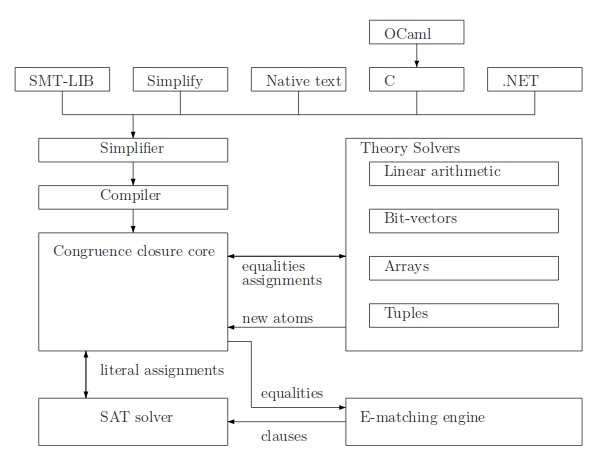
\includegraphics[width=1\textwidth]{arhitektura.png}
  \caption{Arhitektura rešavača Z3}
  \label{fig:arhitektura}
\end{figure}
\par
Formule prosleđene rešavaču se najpre procesiraju upotrebom simplifikacije. Simplifikacija primenjuje algebarska pravila redukcije kao što je \texttt{p $\land$ true $\vdash$ p}. Ovim procesom vrše se i odgovarajuće zamene kao što je \texttt{x=4 $\land$ q(x) $\vdash$ x=4 $\land$ q(4)}.
Nakon simplifikacije, kompajler formira apstraktno sintaksno stablo formula čiji su čvorovi simplifikovane formule (klauze). Zatim se jezgru kongruentnog zatvorenja (eng. 
\textit{Congruence closure core}) prosleđuje apstraktno sintaksno stablo. Jezgro kongruentnog zatvorenja komunicira sa SAT rešavačem koji određuje istinitosnu vrednost klauza. 
\par


Glavni gradivni blokovi formula su konstante, funkcije i relacije. Konstante su specijalan slučaj funkcija bez parametara. Svaka konstanta je određene sorte. Sorta odgovara tipu u programskim jezicima. Relacije su funkcije koje vraćaju povratnu vrednost tipa Boolean. Funkcije mogu uzimati argumente tipa Boolean pa se na taj način relacije mogu koristiti kao argumenti funkcija.  


Formula $F$ je validna ako je vrednost valuacije $true$ za bilo koje interpretacije funkcija i konstantnih simbola. Formula $F$ je zadovoljiva ukoliko postoji bar jedna valuacija u kojoj je formula tačna. Da bismo odredili da li je formula $F$ validna, rešavač Z3 proverava da li je formula $\lnot F$ zadovoljiva. Ukoliko je negacija formule nezadovoljiva, onda je polazna formula validna. 



\section{Teorije} \label{sec:num2}
Teorije rešavača Z3 su opisane u okviru višesortne logike prvog reda sa jednakošću.  Definisanjem specifične teorije, uvode se restrikcije pri definisanju formula kao i podržanih relacija i operatora koje se nad njima primenjuju. Na taj način, specijalizovane metode u odgovarajućoj teoriji mogu biti efikasnije implementirane u poređenju sa opštim slučajem. U nastavku će biti opisane teorija neinterpretiranih funkcija, teorija linearne aritmetike, teorija nelinearne aritmetike, teorija bitvektora i teorija nizova.

\subsection{Teorija neinterpretiranih funkcija}
Teorije obično određuju interpretaciju funkcijskih simbola. Teorija koja ne zadaje nikakva ograničenja za funkcijske simbole naziva se teorija neinterpretiranih funkcija 
(eng. \textit{Theory of Equality with Uninterpreted Functions}, skraćeno EUF). \par Kod rešavača Z3, funkcije i konstantni simboli su neinterpretirani. Ovo je kontrast u odnosu na funkcije odgovarajućih teorija. Funkcija + ima standardnu interpretaciju u teoriji aritmetike. Neinterpretirane funkcije i konstante su maksimalno fleksibilne i dozvoljavaju bilo koju interpretaciju koja je u skladu sa ograničenjima. Za razliku od programskih jezika, funkcije logike prvog reda su totalne, tj. definisane su za sve vrednosti ulaznih parametara. Na primer, deljenje 0 je dozvoljeno, ali nije specifikovano šta ono predstavlja. Teorija neinterpretiranih funkcija je odlučiva i postoji procedura odlučivanja polinomijalne vremenske složenosti. Jedna od procedura odlučivanja za ovu teoriju zasniva se na primeni algoritma Nelson-Open (eng. \textit{Nelson-Open algorithm}). O ovom algoritmu može se više naći u literaturi \cite{NelsonOpen}.
\par



\subsection{Teorija linearne aritmetike} 

Rešavač Z3 sadrži procedure odlučivanja za linearnu aritmetiku nad celobrojnim i realnim brojevima. Dodatni materijali o procedurama odlučivanja linearne aritmetike dostupni su u literaturi \cite{FastLinearArithmetic}.
\par

U okviru celobrojne linearne aritmetike, podržani funkcijski simboli su $+$, $-$ i $*$ pri čemu je kod množenja drugi operand konstanta. Nad funkcijskim simbolima, čiji su specijalni slučajevi konstante mogu se primenjivati relacijski operatori $<$, $\leq$, $>$ i $\geq$. 
\par
U okviru realne linearne aritmetike, podržani funkcijski simboli su $+$, $-$ i $*$ pri čemu je kod operacije množenja drugi operand konstanta. Pored ovih podržane su operacije $div$ i $mod$, uz uslov da je drugi operand konstanta različita od 0. Nad funkcijskim simbolima, čiji su specijalni slučajevi konstante mogu se primenjivati relacijski operatori $<$, $\leq$, $>$ i $\geq$. 
\par
\subsection{Teorija nelinearne aritmetike} 

Formula predstavlja formulu nelinearne aritmetike ako je oblika (* t s), pri čemu t i s nisu linearnog oblika.
Nelinearna celobrojna aritmetika je neodlučiva, tj. ne postoji procedura koja za proizvoljnu formulu vraća zadovoljivost ili nezadovoljivost. U najvećem broju slučajeva, Z3 vraća nepoznat rezultat. Za nelinearne probleme, rešavač Z3 koristi posebne metode odlučivanja zasnovane na Grebnerovim bazama. 


\subsection{Teorija bitvektora} 
Rešavač Z3 podržava bitvektore proizvoljne dužine. \texttt{(\_ BitVec n)} je sorta bitvektora čija je dužina \texttt{n}. Bitvektor literali se mogu definisati koristeći binarnu, decimalnu ili heksadecimalnu notaciju. U binarnom i heksadecimalnom slučaju, veličina bitvektora je određena brojem karaktera. Na primer, literal \textit{\#b010} u binarnom formatu je bitvektor dužine 3. Kako konstanta \textit{a} u heksadecimalnom formatu odgovara vrednosti 10, literal \textit{\#x0a} je bitvektor veličine 10. Veličina bitvektora mora biti specifikovana u decimalnom formatu. Na primer, reprezentacija \textit{(\_ bv10 32)} je bitvektor dužine 32 sa vrednošću 10. Podrazumevano, Z3 predstavlja bitvektore u heksadecimalnom formatu ukoliko je dužina bitvektora umnožak broja 4 a u suprotnom u binarnom formatu. Bitvektor literali mogu biti reprezentovani u decimalnom formatu. Više materijala o procedurama odlučivanja za teoriju bitvektora može se naći u literaturi \cite{DPBitvector}.

Pri korišćenju operatora nad bitvektorima, mora se eksplicitno navesti tip operatora. Zapravo, za svaki operator podržane su dve varijante za rad sa označenenim i neoznačenim operandima. Ovo je kontrast u odnosu na programske jezike u kojima kompajler na osnovu argumenata implicitno određuje tip operacije (označena ili neoznačena varijanta).
\par
U skladu sa prethodno navedenom činjenicom, teorija bitvektora ima na raspolaganju različite verzije aritmetičkih operacija za označene i neoznačene operande. Za rad sa bitvektorima od aritmetičkih operacija definisane su operacije sabiranja, oduzimanja, određivanje negacije (zapisivanja broja u komplementu invertovanjem svih bitova polaznog broja), množenja, izračunavanja modula pri deljenju, šiftovanje u levo kao i označeno i neoznačeno šiftovanje u desno. Podržane su sledeće logičke operacije: disjunkcija, konjunkcija, unarna negacija, negacija konjunkcije i negacija disjunkcije. Definisane su različite relacije nad bitvektorima kao što su $\leq$, $<$, $\geq$ i $>$.



\subsection{Teorija nizova} 
Osnovnu teoriju nizova karakterišu \texttt{select} i \texttt{store} funkcije. 
Funkcijom \texttt{(select a i)} vraća se vrednost na poziciji i u nizu a, dok se funkcijom \texttt{(store a i v)} formira novi niz, identičan nizu a pri čemu se na poziciji i nalazi vrednost v.
Z3 sadrži procedure odlučivanja za osnovnu teoriju nizova.
Dva niza su jednaka ukoliko su vrednosti svih elemenata na odgovarajućim pozicijama jednake.
 

\subsubsection{Konstantni nizovi}

Nizovi sa konstantnim vrednostima mogu se specifikovati koristeći \texttt{const} konstrukciju. Prilikom upotrebe \texttt{const} konstrukcije rešavač Z3 ne može da odluči kog tipa su elementi niza pa se on mora eksplicitno navesti. Interpretacija nizova je slična interpretaciji funkcija. Z3 koristi konstrukciju \texttt{(\_ as-array f)} za određivanje interpretacije niza. Ako je niz a jednak rezultatu konstrukcije \texttt{(\_ as-array f)}, tada za svaki indeks i, vrednost \texttt{(select a i)} odgovara vrednosti \texttt{(f i)}. 


\subsubsection{Primena map funkcije na nizove}
Rešavač Z3 obezbeđuje primenu parametrizovane funkcije \texttt{map} na nizove. Funkcijom \texttt{map} omogućava se primena proizvoljnih funkcija na sve elemente niza.

Nad nizovima se mogu vršiti slične operacije kao i nad skupovima. Rešavač Z3 ima podršku za računanje unije, preseka i razlike dva niza. Ovi operatori se tumače na isti način kao i u teoriji skupova. Za nizove a i b, pomenuti operatori mogu se koristiti navođenjem funkcija:\\
\texttt{(union a b)} ; kreiranje unije dva niza kao skupa \\
\texttt{(intersect a b)} ; kreiranje preseka dva niza kao skupa \\
\texttt{(difference a b)} ; kreiranje razlike dva niza kao skupa

\section{Tipovi podataka} \label{sec:num3}
U okviru rešavača Z3 dostupni su primitivni tipovi podataka, definisanjem konstanti različitih sorti. Neke od najčešće korišćenih su konstante bulovske, celobrojne i realne sorte.
Pored toga, mogu se definisati algebarski tipovi podataka. Algebarski tipovi podataka omogućavaju specifikaciju uobičajnih struktura podataka. Slogovi, torke i skalari (enumeracijski tipovi) spadaju u algebarske tipove podataka. Primena algebarskih tipova podataka može se generalizovati. Mogu se koristiti za specifikovanje konačnih listi, stabala i rekurzivnih struktura. 
\subsubsection{Slogovi}
Slog se specifikuje kao tip podataka sa jednim konstruktorom i proizvoljnim brojem elemenata sloga. Rešavač Z3 ne dozvoljava povećavanje broja argumenata sloga nakon njegovog definisanja. Važi svojstvo da su dva sloga jednaka samo ako su im svi argumenti jednaki.
\subsubsection{Skalari (tipovi enumeracije)}

Sorta skalara je sorta konačnog domena. Elementi konačnog domena se tretiraju kao različite konstante. Na primer, neka je S skalarni tip sa tri vrednosti A, B i C. Moguće je da tri konstante skalarnog tipa S budu različite. Ovo svojstvo ne može važiti u slučaju četiri konstante.


\subsubsection{Rekurzivni tipovi podataka}

Deklaracija rekurzivnog tipa podataka uključuje sebe direktno kao komponentu. Standardni primer rekurzivnog tipa podataka je lista. 
Lista celobrojnih vrednosti sa imenom \texttt{list} može se deklarisati naredbom:\\
\texttt{(declare-datatypes (list (nil) ((head Int) (tail list)))}
\par
Rešavaš Z3 ima ugrađenu podršku za liste korišćenjem ključne reči \texttt{List}.
Prazna lista se definiše korišćenjem klučne reči \texttt{nil} a konstruktor \texttt{insert} se koristi za dodavanje elemenata u listu. Selektori \texttt{head} i \texttt{tail} se definišu na uobičajan način.


\section{Upotreba rešavača korišćenjem SMT-LIB standarda} \label{sec:num4}
Ulazni format rešavača Z3 je definisan SMT-LIB 2.0 standardom \cite{SMTLIB}. Standard definiše jezik logičkih formula čija se zadovoljivost proverava u odnosu na neku teoriju. Cilj standarda je pojednostavljivanje jezika logičkih formula povećavanjem njihove izražajnosti i fleksibilnosti kao i obezbeđivanje zajedničkog jezika za sve SMT rešavače. 
\par
Interno, Z3 održava stek korisnički definisanih formula i deklaracija. Formule i deklaracije jednim imenom nazivamo tvrđenjima. Komandom \texttt{push} kreira se novi opseg i čuva se trenutna veličina steka. Komandom \texttt{pop} uklanjaju se sva tvrđenja i deklaracije zadate posle push-a sa kojim se komanda uparuje. Komandom \texttt{assert} dodaje se formula na interni stek. Skup formula na steku je zadovoljiv ako postoji interpretacija u kojoj sve formule imaju istinitosnu vrednost tačno. Ova provera se vrši komandom \texttt{check-sat}. U slučaju zadovoljivosti vraća se \texttt{sat}, u slučaju nezadovoljivosti vraća se \texttt{unsat} a kada rešavač ne može da proceni da li je formula zadovoljiva ili ne vraća se \texttt{unknown}. Komandom \texttt{get-model} vraća se interpretacija u kojoj su sve formule na steku tačne. 
\par

Komandom \texttt{declare-const} deklariše se konstanta odgovarajuće sorte. Sorta može biti parametrizovana i u tom slučaju su specifikovana imena njenih parametara. Naredbom \texttt{(define-sort [symbol] ([symbol]+)[sort])} vrši se specifikacija sorte.
Komandom \texttt{declare-fun} deklariše se funkcija. 
U primeru \ref{example1} koristimo činjenicu da se validnost formule pokazuje ispitivanjem zadovoljivosti negirane formule. 

\begin{primer} \label{example1} Dokazivanje de Morganovog zakona dualnosti\label{primer:demorgan} ispitivanjem validnosti formule: $\neg{(a \land b)} \Leftrightarrow (\neg{a} \lor \neg{b}) $ tako što se kao ograničenje dodaje negacija polazne formule. Z3 pronalazi da je negacija formule nezadovoljiva, pa je polazna formula tačna u svim interpretacijama. \\

\hspace{-0.6cm}
\begin{minipage}[b]{0.5\textwidth}
\textbf{Formula prosleđena rešavaču:}
\\(declare-const a Bool)
\\(declare-const b Bool)
\\(define-fun demorgan () Bool
\\\tab (= (and a b) (not (or (not a) (not b))))
\\)
\\(assert (not demorgan))
\\(check-sat) 
\\(get-model)
\end{minipage}
\hspace{1.5cm}
\begin{minipage}[t]{0.4\textwidth}
\vspace{-5.35cm}
\textbf{Izlaz:}
\\unsat
\end{minipage}
\end{primer}

Rešavač Z3 ima podršku za celobrojne i realne konstante. Komandom \texttt{declare-const} deklarišu se celobrojne i realne konstante. Rešavač ne vrši automatsku konverziju između celobrojnih i realnih konstanti. Ukoliko je potrebno izvršiti ovakvu konverziju koristi se funkcija \texttt{to-real} za konvertovanje celobrojnih u realne vrednosti.
Realne konstante treba da budu zapisane sa decimalnom tačkom. Primer \ref{example2} ilustruje deklarisanje konstanti i funkcija kao i primenu funkcije na konstante. Ispituje se zadovoljivost ograničenja.

\begin{primer} \label{example2} 
Rešavaču se prosleđuje ograničenja koje sadrže primenu funkcije f na celobrojnu konstantu a kao i relacijske operatore. Rešavač Z3 pronalazi da je ovo tvrđenje zadovoljivo i daje prikazani model. 
\\ 

\hspace{-0.7cm}
\begin{minipage}[b]{0.43\textwidth}
\textbf{Formula prosleđena rešavaču:}\\
(declare-const a Int)\\
(declare-fun f (Int Bool) Int)\\
(assert (> a 10))\\
(assert (< (f a true) 100))\\
(check-sat)\\
(get-model) \\
\end{minipage}
\hspace{0.6cm}
\begin{minipage}[t]{0.5\textwidth}
\vspace{-4.715cm}
\textbf{Izlaz:}
\\sat 
\\(model 
\\\tab(define-fun a () Int 11) 
\\\tab(define-fun f ((x!1 Int) (x!2 Bool)) Int 
\\\tab(ite (and (= x!1 11) (= x!2 true)) 0 0))
\\)
\end{minipage}
\end{primer}

Primer \ref{example3} ilustruje pronalaženje interpretacija celobrojnih i realnih konstanti. Interpretacija se svodi na pridruživanje brojeva svakoj konstanti. 

\begin{primer} \label{example3} 
Rešavaču se prosleđuju jednostavna ograničenja za celobrojne i realne konstante.
Ograničenja sadrže aritmetičke i relacijske operatore. Rešavač vraća zadovoljivost tvrđenja i dobijeni model prikazujemo u nastavku.\\ \\
\begin{minipage}[b]{0.47\textwidth}
\textbf{Formula prosleđena rešavaču:}
\\(declare-const a Int)
\\(declare-const b Int)
\\(declare-const c Int)
\\(declare-const d Real)
\\(declare-const e Real)
\\(assert (> e (+ (to\_real (+ a b)) 2.0)))
\\(assert (= d (+ (to\_real c) 0.5)))
\\(check-sat)
\\(get-model)
\end{minipage}
\hspace{1.6cm}
\begin{minipage}[t]{0.4\textwidth}
\vspace{-6cm}
\textbf{Izlaz:}
\\sat 
\\(model
\\\tab(define-fun b () Int 0) 
\\\tab(define-fun a () Int 1) 
\\\tab(define-fun e () Real 4.0) 
\\\tab(define-fun c () Int 0) 
\\\tab(define-fun d () Real (/ 1.0 
\\\tab 2.0))
\\)
\end{minipage}

\end{primer}


Takođe, postoji uslovni operator (if-then-else operator). Na primer,
izraz (ite (and (= x!1 11) (= x!2 false)) 21 0) ima vrednost 21 kada je promenljiva x!1 jednaka 11, a promenljiva x!2 ima vrednost False. U suprotnom, vraća se 0.

U slučaju deljenja, može se koristiti \texttt{ite} (if-then-else) operator i na taj način se može dodeliti interpretacija u slučaju deljenja nulom.
\par
Mogu se konstruisati novi operatori, korišćenjem \texttt{define-fun} konstruktora. Ovo je zapravo makro, pa će rešavač vršiti odgovarajuće zamene. U primeru \ref{example4} ilustruje se definisanje novog operatora. Zatim se novi operator primenjuje na konstante, uvode se ograničenja i ispituje njihova zadovoljivost.
\begin{primer} \label{example4}
Definišemo operator deljenja tako da rezultat bude specifikovan i kada je delilac 0. Uvode se dve konstante realnog tipa i primenjuje se definisani operator. Z3 rešavač pronalazi nezadovoljivost tvrđenja s obzirom da operator \texttt{mydiv} vraća 0 pa relacija poređenja ne može biti tačna.\\ \\
\begin{minipage}[b]{0.5\textwidth}
\textbf{Formula prosleđena rešavaču:}
\\(define-fun mydiv ((x Real) (y Real)) Real
\\\tab (if (not (= y 0.0))  (/ x y)  0.0))
\\(declare-const a Real)
\\(declare-const b Real)
\\(assert (>= (mydiv a b) 1.0))
\\(assert (= b 0.0))
\\(check-sat)
\end{minipage}
\hspace{3cm}
\begin{minipage}[t]{0.4\textwidth}
\vspace{-4.73cm}
\textbf{Izlaz:}
\\unsat
\end{minipage}
\end{primer}
\par
Primer \ref{example5} ilustruje rešavanje nelinearnog problema uvođenjem ograničenja nad realnim konstantama. Ispituje se zadovoljivost prosleđenih ograničenja. Kada su prisutna samo nelinearna ograničenja nad realnim konstantama, Z3 koristi posebne metode odlučivanja\begin{primer} \label{example5} Rešavaču se prosleđuje ograničenja $b^{3} + b*c = 3$ nad realnim konstantama. Rešavač vraća zadovoljivost tvrđenja i dobijeni model prikazujemo u nastavku.   
\\ \\
\begin{minipage}[b]{0.43\textwidth}
\textbf{Formula prosleđena rešavaču:}
\\(declare-const b Real)
\\(declare-const c Real)
\\(assert (= (+ (* b b b) (* b c)) 3.0))
\\(check-sat)
\\(get-model)

\end{minipage}
\hspace{1.5cm}
\begin{minipage}[t]{0.45\textwidth}
\vspace{-3.4cm}
\textbf{Izlaz:}
\\sat 
\\(model 
\\\tab(define-fun b () Real (/ 1.0 8.0)) 
\\\tab(define-fun c () Real (/ 15.0 64.0))
\\)
\end{minipage}
\end{primer}
\par
Primer \ref{example6} ilustruje različite načine predstavljanja bitvektora. Ukoliko zapis počinje sa \#b, bitvektor se zapisuje u binarnom formatu. Ukoliko zapis počinje sa \#x, bitvektor se zapisuje u heksadecimalnom formatu.
\begin{primer} \label{example6} 
Nakon specifikacije formata, zapisuje se dužina vektora. Drugi način zapisa počinje skraćenicom \texttt{bv}, navođenjem vrednosti i na kraju dužine. Komandom \texttt{(display t)} štampa se izraz \texttt{t}.\\\\
\begin{minipage}[b]{0.45\textwidth}
\textbf{Formula prosleđena rešavaču:}
\\(display \#b0100)
\\(display (\_ bv20 8))
\\(display (\_ bv20 7))
\\(display \#x0a) 
\\(set-option :pp.bv-literals false)
\\(display \#b0100)
\\(display (\_ bv20 8))
\\(display (\_ bv20 7))
\\(display \#x0a)
\end{minipage}
\hspace{2.5cm}
\begin{minipage}[t]{0.4\textwidth}
\vspace{-5.93cm}
\textbf{Izlaz:}
\\\#x4 
\\\#x14 
\\\#b0010100 
\\\#x0a 
\\(\_ bv4 4) 
\\(\_ bv20 8) 
\\(\_ bv20 7) 
\\(\_ bv10 8)
\end{minipage}
\end{primer}
\par Primer \ref{example7} ilustruje primenu aritmetičkih operacija nad bitvektorima. Podržane aritmetičke operacije su sabiranje \texttt{(bvadd)}, oduzimanje \texttt{(bvsub)}, unarna negacija \texttt{(bvneg)}, množenje \texttt{(bvmul)}, računanje modula \texttt{(bvmod)}, šiftovanje ulevo \texttt{(bvshl)}, neoznačeno (logičko) šiftovanje udesno \texttt{(bvlshr)} i označeno (aritmetičko) šiftovanje udesno \texttt{(bvashr)}. Od logičkih operacija postoji podrška za disjunkciju \texttt{(bvor)}, konjunkciju \texttt{(bvand)}, ekskluzivnu disjunkciju \texttt{(bvxor)}, negaciju disjunkcije \texttt{(bvnor)}, negaciju konjunkcije \texttt{(bvnand)} i negaciju ekskluzivne disjunkcije \texttt{(bvnxor)}.
\begin{primer} \label{example7} 
Ovaj primer ilustruje primenu nekih aritmetičkih operacija nad bitvektorima i dobijene rezultate. Komandom \texttt{(simplify t)} prikazuje se jednostavniji izraz ekvivalentan izrazu \texttt{t} ukoliko postoji.
\\ \\
\begin{minipage}[b]{0.5\textwidth}
\textbf{Formula prosleđena rešavaču:}
\\(simplify (bvadd \#x07 \#x03)) 
\\(simplify (bvsub \#x07 \#x03)) 
\\(simplify (bvneg \#x07))       
\\(simplify (bvmul \#x07 \#x03)) 
\\(simplify (bvsmod \#x07 \#x03)) 
\\(simplify (bvshl \#x07 \#x03)) 
\\(simplify (bvlshr \#xf0 \#x03))  
\\(simplify (bvashr \#xf0 \#x03))  
\\(simplify (bvor \#x6 \#x3)) 
\\(simplify (bvand \#x6 \#x3))   
\end{minipage}
\hspace{2.5cm}
\begin{minipage}[b]{0.5\textwidth}
\textbf{Izlaz:}
\\\#x0a 
\\\#x04 
\\\#xf9 
\\\#x15 
\\\#x01 
\\\#x38 
\\\#x1e 
\\\#xfe
\\\#x7 
\\\#x2 
\end{minipage}

\end{primer} \par
Postoji brz način da se proveri da li su brojevi fiksne dužine stepeni dvojke. U primeru \ref{example8} pokazuje se da je bitvektor x stepen dvojke ako i samo ako je vrednost izraza x $\land$ (x - 1) jednaka 0.

\begin{primer} \label{example8}
Provera da li je broj stepen dvojke primenjuje se na bitvektore čije su vrednosti 0, 1, 2, 4 i 8. Rešavaču se prosleđuje negacija formule. U svim slučajevima brojevi su stepeni dvojke pa Z3 rešavač vraća nezadovoljivost.\\ \\
\begin{minipage}[b]{0.5\textwidth}
\textbf{Formula prosleđena rešavaču:}
\\(define-fun is-power-of-two 
\\\tab((x (\_ BitVec 4))) Bool 
\\\tab(= \#x0 (bvand x (bvsub x \#x1)))
\\)
\\(declare-const a (\_ BitVec 4))
\\(assert 
\\\tab(not (= (is-power-of-two a) 
\\\tab\tab    (or (= a \#x0) 
\\\tab\tab\tab     (= a \#x1) 
\\\tab\tab\tab     (= a \#x2) 
\\\tab\tab\tab     (= a \#x4) 
\\\tab\tab\tab     (= a \#x8)
\\\tab\tab		))
\\\tab )
\\)
\\(check-sat)
\end{minipage}
\hspace{2.5cm}
\begin{minipage}[t]{0.5\textwidth}
\vspace{-10.45cm}
\textbf{Izlaz:}
\\unsat
\end{minipage}
\end{primer}
\par Primer \ref{example9} ilustruje upotrebu relacija nad bitvektorima. Podržane relacije uključuju neoznačene i označene verzije za operatore $<$, $\leq$, $>$ i $\geq$. Neoznačene varijante počinju nazivom \texttt{bvu}, a u nastavku sledi ime relacije. Označene varijante počinju nazivom \texttt{bvs}, a u nastavku ponovo sledi ime relacije. 
\begin{primer} \label{example9} Primer ilustruje upotrebu označenih i neoznačenih verzija operatora nad bitvektorima. Na primer, relacija $\leq$ nad neoznačenim brojevima zadaje se komandom \texttt{bvule}, a relacija $>$ nad neoznačenim brojevima komandom \texttt{bvugt}. Slično, relacija $\geq$ nad neoznačenim brojevima zadaje se komandom \texttt{bvsge}, a relacija $<$ nad označenim brojevima komandom \texttt{bvslt}.
\\ \\ 
\begin{minipage}[b]{0.5\textwidth}
\textbf{Formula prosleđena rešavaču:}
\\(simplify (bvule \#x0a \#xf0))  
\\(simplify (bvult \#x0a \#xf0))  
\\(simplify (bvuge \#x0a \#xf0))  
\\(simplify (bvugt \#x0a \#xf0))  
\\(simplify (bvsle \#x0a \#xf0)) 
\\(simplify (bvslt \#x0a \#xf0))  
\\(simplify (bvsge \#x0a \#xf0))  
\\(simplify (bvsgt \#x0a \#xf0))

\end{minipage}
\hspace{2cm} 
\begin{minipage}[t]{0.5\textwidth}
\vspace{-5.3cm}
\textbf{Izlaz:}
\\true 
\\true 
\\false 
\\false 
\\false 
\\false 
\\true 
\\true
\end{minipage}


\end{primer}

Rešavač Z3 nudi funkcije za promenu načina reprezentacije brojeva. Moguće su konverzije reprezentacije brojeva linearne aritmetike u reprezentaciju bitvektora i obrnuto. Ovaj rezultat može se postići naredbama: \\
\texttt{(define b (int2bv[32] z))} \\  
\texttt{(define c (bv2int[Int] x))}
\par
Primer \ref{example10} ilustruje poređenje bitvektora koristeći označene i neoznačene verzije operatora. Ispituje se zadovoljivost prosleđenog ograničenja.
\begin{primer} \label{example10} Označeno poređenje, kao što je bvsle, uzima u obzir znak bitvektora za poređenje, dok neoznačeno poređenje komandom bvule tretira bitvektor kao prirodan broj. Z3 rešavač pronalazi da je tvrđenje zadovoljivo i daje prikazani model.
\\ \\
\begin{minipage}[b]{0.5\textwidth}
\textbf{Formula prosleđena rešavaču:}
\\(declare-const a (\_ BitVec 4))
\\(declare-const b (\_ BitVec 4))
\\(assert (not (= (bvule a b) (bvsle a b)))
\\(check-sat)
\\(get-model)
\end{minipage}
\hspace{1.15cm} 
\begin{minipage}[t]{0.5\textwidth}
\vspace{-3.45cm}
\textbf{Izlaz:}
\\sat 
\\(model 
\\\tab(define-fun b () (\_ BitVec 4) \#xe) 
\\\tab(define-fun a () (\_ BitVec 4) \#x0)
\\)
\end{minipage}
\end{primer}
\par
Primer \ref{example11} ilustruje kako se definišu nizovi sa konstantnim vrednostima. Zatim se dodaju ograničenja korišćenjem funkcije \texttt{select} i ispituje se njihova zadovoljivost.
\begin{primer} \label{example11} Definišemo konstantni niz m celobrojnog tipa i dve celobrojne konstante a i i. Uvodimo ograničenje da niz m sadrži samo jedinice. Z3 pronalazi da je ovo tvrđenje zadovoljivo i daje prikazani model.\\
\begin{minipage}[b]{0.55\textwidth}
\vspace{0.5cm} 
\textbf{Formula prosleđena rešavaču:}
\\(declare-const m (Array Int Int))
\\(declare-const a Int)
\\(declare-const i Int)
\\(assert (= m ((as const (Array Int Int)) 1)))
\\(assert (= a (select m i)))
\\(check-sat)
\\(get-model)
\end{minipage}
\hspace{1.1cm} 
\begin{minipage}[t]{0.5\textwidth}
\vspace{-4.7cm}
\textbf{Izlaz:}
\\sat 
\\(model 
\\\tab(define-fun m () (Array Int Int) 
\\\tab\tab(\_ as-array k!0)
\\\tab) 
\\\tab(define-fun i () Int 0) 
\\\tab(define-fun a () Int 1) 
\\\tab(define-fun k!0 ((x!0 Int)) 
\\\tab\tab Int (ite (= x!0 0) 1 1)
\\\tab)
\\)
\end{minipage}
\end{primer}
\par
Primer \ref{example12} ilustruje primenu funkcije \texttt{map} na sve elemente konstatnih nizova. Za svaka dva elementa koji pripadaju različitim nizovima, pokazuje se važenje De Morganovog zakona iz primera \ref{example1}. 
\begin{primer} \label{example12} 
Kao ograničenje dodajemo negaciju navedene formule. Rešavač Z3 vraća nezadovoljivost negirane formule, odakle zaključujemo da je polazna formula validna.\\ \\
\begin{minipage}[b]{0.65\textwidth}
\textbf{Formula prosleđena rešavaču:}
\\(define-sort Set (T) (Array T Bool))
\\(declare-const a (Set Int))
\\(declare-const b (Set Int))
\\(assert (not (= ((\_ map and) a b) ((\_ map not) 
\\\tab((\_ map or) ((\_ map not) b) ((\_ map not) a)))))
\\)
\\(check-sat)
\end{minipage}
\hspace{2.5cm} 
\begin{minipage}[t]{0.5\textwidth}
\vspace{-4.65cm}
\textbf{Izlaz:}
\\unsat 
\end{minipage}
\end{primer}

\par
U primeru \ref{example13} pokazuje se da su dva sloga jednaka ako i samo ako su im svi argumenti jednaki. Uvodi se parametarski tip \texttt{Pair} i koriste se selektorske funkcije \texttt{first} i \texttt{second}. 

\begin{primer} \label{example13} Nakon definisanja slogova p1 i p2, dodaje se ograničenje koje se odnosi na drugi element sloga.
Dodajemo i ograničenje da su slogovi p1 i p2 jednaki. Rešavač Z3 vraća zadovoljivost formule i odgovarajući model. 
\\ \\
\begin{minipage}[b]{0.5\textwidth}
\textbf{Formula prosleđena rešavaču:}
\\(declare-datatypes (T1 T2) 
\\\tab[0.3cm](Pair (mk-pair (first T1) (second T2))))
\\(declare-const p1 (Pair Int Int))
\\(declare-const p2 (Pair Int Int))
\\(assert (= p1 p2))
\\(assert (> (second p1) 20))
\\(check-sat)
\\(get-model)
\end{minipage}
\hspace{1.5cm} 
\begin{minipage}[t]{0.5\textwidth}
\vspace{-5.35cm}
\textbf{Izlaz:}
\\sat 
\\(model 
\\\tab(define-fun p1 () (Pair Int Int) 
\\\tab\tab(mk-pair 0 21)
\\\tab) 
\\\tab(define-fun p2 () (Pair Int Int) 
\\\tab\tab(mk-pair 0 21)
\\\tab)
\end{minipage}

\end{primer}
\par
U primeru \ref{example14} ilustruje se definisanje listi kao i dodavanje ograničenja korišćenjem selektorskih funkcija \texttt{head} i \texttt{tail}. Ispituje se zadovoljivost tvrđenja.
\begin{primer} \label{example14}
Pored ograničenja za prve elemente listi, tražimo model takav da liste l1 i l2 nisu jednake, tj. da nisu svi elementi na odgovarajućim pozicijama u listama jednaki. Rešavač Z3 vraća zadovoljivost tvrđenja i dobijeni model prikazujemo u nastavku.
\\ \\
\begin{minipage}[b]{0.42\textwidth}
\textbf{Formula prosleđena rešavaču:}
\\(declare-const l1 (List Int))
\\(declare-const l2 (List Int))
\\(declare-const l3 (List Int))
\\(declare-const x Int)
\\(assert (not (= l1 nil)))
\\(assert (not (= l2 nil)))
\\(assert (= (head l1) (tail l2)))
\\(assert (not (= l1 l2)))
\\(assert (= l3 (insert x l2)))
\\(assert (> x 100))
\\(check-sat)
\\(get-model)
\end{minipage}
\hspace{0.9cm}
\begin{minipage}[t]{0.55\textwidth}
\vspace{-7.84cm}
\textbf{Izlaz:}
\\sat 
\\(model 
\\\tab(define-fun l3 () (List Int) 
\\\tab(insert 101 (insert 0 (insert 1 nil)))
\\\tab(define-fun x () Int 101) 
\\\tab(define-fun l1 () (List Int) (insert 0 nil)) 
\\\tab(define-fun l2 () (List Int) (insert 0 
\\\tab\tab(insert 1 nil))
\\\tab)
\\) 
\end{minipage}


\end{primer}

U prethodnom primeru, uvode se ograničenja da su liste l1 i l2 različite od \texttt{nil}. Ova ograničenja se uvode jer interpretacija selektora \texttt{head} i \texttt{tail} 
nije specifikovana u slučaju praznih lista.



\section{Upotreba rešavača korišćenjem C++ interfejsa} \label{sec:num5}
C++ interfejs prema rešavaču Z3 obezbeđuje različite strukture podataka, klase i funkcije koje su potrebne za direktnu komunikaciju C++ aplikacije sa rešavačem. Neke od najbitnijih klasa biće opisane u nastavku, dok se kompletan opis interfejsa može naći na internetu \cite{cppapi}.

Klasa \texttt{Z3\_sort} koristi se za definisanje sorte izraza.  Prilikom definisanja izraza navodi se sorta kako bi bio poznat skup vrednosti koje mu se mogu dodeliti kao i skup dozvoljenih metoda. Sorte izraza definisane su tipom enumeracije. Neke od najvažnijih sorti su \texttt{Z3\_BOOL\_SORT}, \texttt{Z3\_INT\_SORT}, \texttt{Z3\_REAL\_SORT}, \texttt{Z3\_BV\_SORT} i \texttt{Z3\_ARRAY\_SORT}. Određivanje sorte izraza vrši se funkcijom \texttt{sort\_kind()} sa povratnom vrednošću tipa enumeracije. Za proveru pripadnosti izraza sorti, koriste se funkcije \texttt{is\_bool()}, \texttt{is\_int()}, \texttt{is\_real()}, \texttt{is\_array()} i \texttt{is\_bv()}. Sorte različitih izraza se mogu porediti korišćenjem operatora jednakosti. \par 

Za upravljanje objektima interfejsa kao i za globalno konfigurisanje koristi se klasa \texttt{context}. Klasa sadrži konstruktor bez argumenata. Upotrebom klase \texttt{context}, mogu se detektovati različite vrste grešaka u korišćenju C++ API-ja. Greške su definisane tipom enumeracije \texttt{Z3\_ERROR\_CODE}. Neke od konstanti enumeracije su \texttt{Z3\_OK}, \texttt{Z3\_SORT\_ERROR}, \texttt{Z3\_INVALID\_USAGE} i \texttt{Z3\_INTERNAL\_FATAL}.  Kontekst omogućava kreiranje konstanti metodama \texttt{bool\_const()}, \texttt{int\_const()}, \texttt{real\_const()} i \texttt{bv\_const()}. Definisanje različitih sorti omogućeno je metodama \texttt{bool\_sort()}, \texttt{int\_sort()}, \texttt{real\_sort()}, \texttt{bv\_sort()} i \texttt{array\_sort()}. 
\par

Izrazi koji se formiraju pripadaju klasi \texttt{expr}. Sadrži konstruktor čiji je argument objekat klase \texttt{context}. Za dobijanje izraza na zadatoj poziciji u skupu izraza koristi se metoda \texttt{at(expr const \&index)}.  Provera da li podizraz predstavlja deo drugog izraza vrši se metodom  \texttt{contains(expr const \&s)}. Za dobijanje pojednostavljenog izraza ekvivalentnog polaznom koristi se metoda \texttt{simplify()} ukoliko takav izraz postoji. Za dobijanje pojednostavljenog izraza može se navesti i skup parametara koji se prosleđuju Z3 simplifikatoru. Zamenu vektora izraza drugim vektorom vrši se metodom \texttt{substitute(expr\_vector const \&source, expr\_vector const \&destination)}. 
\par
Postoji veliki broj metoda i operatora koji se koriste za izgradnju složenih izraza. Podržan je veliki broj aritmetičkih operatora za rad za izrazima uključujući operatore sabiranja, oduzimanja, množenja, deljenja, računanja stepena i modula. Svi aritmetički operatori kao argumente imaju izraze. Rezultat primene operatora je novi izraz. Pored toga, mogu se koristiti i različiti logički operatori. Neke od podržanih logičkih operacija su konjunkcija, disjunkcija, implikacija, negacija konjunkcije i negacija disjunkcije. Konjunkcija vektora izraza vrši se metodom \texttt{mk\_and(expr\_vector const \&args)}. Disjunkcija vektora izraza vrši se metodom \texttt{mk\_or(expr\_vector const \&args)}. Implikacija dva izraza vrši se metodom \texttt{implies(expr const \&a, expr const \&b)}. Negacija konjunkcije dva izraza vrši se metodom \texttt{nand(expr const  \&a, expr const \&b)}. Negacija disjunkcije dva izraza vrši se metodom \texttt{nor(expr const \&a, expr const \&b)}. Nad izrazima se mogu primenjivati relacijski operatori \texttt{==}, \texttt{!=}, \texttt{<}, \texttt{<=}, \texttt{>}, \texttt{>=} pri čemu izrazi moraju biti odgovarajuće sorte kako bi poređenje bilo moguće. Nadovezivanje dva izraza vrši se metodom \texttt{concat(expr const \&a, expr const \&b)}. Može se vršiti i nadovezivanje vektora izraza. Kombinovanjem pomenutih metoda i operatora mogu se graditi izrazi proizvoljne složenosti. 	
\par
Definicija funkcije vrši se objektima klase \texttt{func\_decl}. Korišćenjem ove klase definišu se interpretirane i neinterpretirane funkcije rešavača Z3. 
Povratne vrednosti funkcija određene su tipom enumeracije \texttt{Z3\_decl\_kind}. Neke od konstanti enumeracije su \texttt{Z3\_OP\_TRUE}, \texttt{Z3\_OP\_FALSE}, \texttt{Z3\_OP\_REAL}, \texttt{Z3\_OP\_INT} i \texttt{Z3\_OP\_ARRAY}. Dobijanje imena funkcijskog simbola vrši se metodom \texttt{name()}. Određivanje arnosti funkcijskog simbola vrši se metodom \texttt{arity()}. Određivanje sorte i-tog parametra funkcijskog simbola određuje se metodom \texttt{domain(unsigned i)}. 
\par


U okviru C++ interfejsa, teorije rešavača Z3 zadate su semantički navođenjem modela. Ova podrška implementirana je klasom \texttt{model}. Sadrži konstruktor čiji je argument objekat klase \texttt{context}. Interpretacija izraza definisanog u modelu dobija se korišćenjem metode \texttt{eval(expr const \&n)}. Metodom \texttt{get\_func\_decl(unsigned i)} dobija se i-ti funkcijski simbol modela.  
Metodom \texttt{get\_const\_decl(unsigned i)} dobija se interpretacija i-te konstante modela. Metodom \texttt{num\_consts()} dobija se broj konstanti datog modela kao funkcijskih simbola arnosti 0. Metodom \texttt{num\_funcs()} dobija se broj funkcijskih simbola arnosti veće od 0.  Metodom \texttt{size()} vraća se broj funkcijskih simbola modela. Poređenje modela vrši se operatorom jednakosti. Dva modela su jednaka ukoliko su im jednake interpretacije svih funkcijskih simbola. Za ispisivanje modela, koristi se funkcija \texttt{Z3\_model\_to\_string} čiji su argumenti objekti klasa \texttt{context} i \texttt{model}.\par 


Sa Z3 rešavačem komunicira se korišćenjem objekta klase \texttt{solver}. Objekat klase \texttt{solver} inicijalizuje se vrednostima objekta klase \texttt{context}. Osnovni metodi klase solver su \texttt{add}, \texttt{check} i \texttt{get\_model}. Metodom \texttt{add(expr const \&e)} dodaje se ograničenje koje se prosleđuje rešavaču. Metodom \texttt{check()} proverava se zadovoljivost ograničenja prosleđenih rešavaču. Metodom \texttt{get\_model()} vraća se model definisan ograničenjima ukoliko postoji. Pre korišćenja metode \texttt{get\_model()}, mora se pozvati metod \texttt{check()}. Metodom \texttt{assertions()} vraća se vektor ograničenja prosleđenih rešavaču. Ograničenja se mogu čitati iz fajla i iz stringa, korišćenjem metoda \texttt{from\_file(char const *file)} i \texttt{from\_string(char const *s)}. Uklanjanje svih ograničenja prosleđenih rešavaču vrši se metodom \texttt{reset()}. \par

\subsection{Interfejs kroz primere}
Naredni primeri ilustruju korišćenje najvažnijih klasa i metoda C++ interfejsa za komunikaciju sa Z3 rešavačem. Primer \ref{ex1} ilustruje kreiranje bulovskih izraza i jednostavne formule i prikazuje kako se kreira i upotrebljava klasa \texttt{context} i klasa \texttt{solver}. U ovom primeru, ilustrovano je dodavanje ograničenja u solver metodom \texttt{add} i proveravanje njegove zadovoljivosti metodom \texttt{check}. 

\begin{primer} \label{ex1} Primer demonstrira važenje De Morganovog zakona dokazivanjem formule iz primera \ref{primer:demorgan}. Pokazuje se nezadovoljivost negirane formule. U zavisnosti od rezultata štampa se odgovarajuća poruka.
\begin{lstlisting}[language=C++]
void demorgan() {
    context c;
    expr x = c.bool_const("x");
    expr y = c.bool_const("y");
    expr e = (!(x && y)) == (!x || !y);
    
    solver s(c);
    s.add(!e);

    switch (s.check()) {
    case unsat:   std::cout << "Formula je validna"; break;
    case sat:     std::cout << "Formula nije validna"; break;
    case unknown: std::cout << "Rezultat je nepoznat"; break;
    }
}
\end{lstlisting}
\end{primer}

Primer \ref{ex2} ilustruje kreiranje celobrojnih konstanti i jednostavne neinterpretirane funkcije upotrebom klase \texttt{func\_decl}. Prilikom definisanja funkcije navodi se njeno ime kao i sorte argumenta i povratne vrednosti. Ilustruje se kreiranje složenijeg izraza upotrebom metode \texttt{implies} koji odgovara logičkom operatoru implikacije. Složeniji izraz prosleđuje se solveru i proverava se njegova zadovoljivost.
\begin{primer} \label{ex2} Primer demonstrira upotrebu neinterpretiranih funkcija dokazivanjem formule x = y => g(x) = g(y). Dodaje se negacija prethodno navedene formule. U zavisnosti od rezultata, štampa se odgovarajuća poruka.\\
\begin{lstlisting}[language=C++]
void primer_sa_neinterpretiranim_funkcijama() { 
    context c;
    expr x      = c.int_const("x");
    expr y      = c.int_const("y");
    sort I      = c.int_sort();
    func_decl g = function("g", I, I);
    
    solver s(c);
    expr e = implies(x == y, g(x) == g(y));
    s.add(!e);
    if (s.check() == unsat) 
        std::cout << "dokazano";
    else
        std::cout << "nije dokazano";
}
\end{lstlisting}
\end{primer}
\par
U primeru \ref{ex3} korišćenjem metode \texttt{get\_model} pristupa se modelu koji je solver vratio. Vrši se evaluacija izraza dobijenih iz modela primenom metode \texttt{eval}.  
\begin{primer} \label{ex3} Rešavaču se prosleđuju jednostavna ograničenja nad konstantama. Zatim se vrši evaluacija jednostavnih izraza nad konstantama definisanih u modelu.
\begin{lstlisting}[language=C++]
void eval_primer() {
    context c;
    expr x = c.int_const("x");
    expr y = c.int_const("y");
    solver s(c);

    s.add(x < y);
    s.add(x > 2);
    std::cout << s.check();
    
    model m = s.get_model();
    std::cout << "Model:" << m;
    std::cout << "x+y = " << m.eval(x+y);
}
\end{lstlisting}
\end{primer}


Primer \ref{ex4} ilustruje pronalaženje interpretacija konstanti modela za problem linearne aritmetike uvođenjem ograničenja.
Pokazuje se kako se korišćenjem klase \texttt{func\_decl} pristupa konstantama modela kao funkcijskim simbolima arnosti 0.
\begin{primer} \label{ex4}
Rešavaču se prosleđuju jednostavna ograničenja linearne aritmetike $x >= 1$  i $y < x + 3$. Ispisuju se imena i interpretacije konstanti modela korišćenjem
funkcije \texttt{arity} klase \texttt{func\_decl}.
\\
\begin{lstlisting}[language=C++]
void primer_linearne_aritmetike() {
    context c;
    expr x = c.int_const("x");
    expr y = c.int_const("y");
    solver s(c);
    s.add(x >= 1);
    s.add(y < x + 3);
    model m = s.get_model();

    for(unsigned i = 0; i < m.size(); i++) {
        func_decl v = m[i];
        assert(v.arity() == 0); 
        std::cout << v.name() << "=" << m.get_const_interp(v);
    }
}
\end{lstlisting}
\end{primer}

Primer \ref{ex5} ilustruje pronalaženje interpretacija realnih konstanti modela za problem nelinearne aritmetike uvođenjem ograničenja. Interpretacija realnih konstanti ispisuje se u celobrojnom i realnom formatu korišćenjem opcija za konfigurisanje formata ispisa klase \texttt{context}. 

\begin{primer} \label{ex5}
Rešavaču se prosleđuju jednostavna ograničenja nelinearne aritmetike 
$x^2 + y^2 = 1$ i $x^3 + z^3 < 0.5$. Ispisuju se imena i interpretacije konstanti modela korišćenjem funkcije \texttt{arity} klase \texttt{func\_decl}.
\\
\begin{lstlisting}[language=C++]
void primer_nelinearne_aritmetike() {    
    context c;
    expr x = c.real_const("x");
    expr y = c.real_const("y");
    expr z = c.real_const("z");
                     
    solver s(c);
    s.add(x*x + y*y == 1);                    
    s.add(x*x*x + z*z*z < c.real_val("1/2"));  
    
    std::cout << s.check();
    model m = s.get_model();
    std::cout << m;
    
    for(unsigned i = 0; i < m.size(); i++) {
        func_decl v = m[i];
        assert(v.arity() == 0); 
        std::cout << v.name() << "=" << m.get_const_interp(v);
    }

}
\end{lstlisting}
\end{primer}


Primer \ref{ex6} ilustruje pronalaženje interpretacija konstanti koje imaju bitvektorsku reprezentaciju korišćenjem metode \texttt{bv\_const} klase \texttt{context}. Parametri ove metode su ime i broj mesta za zapisivanje konstante. 
\begin{primer} \label{ex6} 
Rešavaču se prosleđuje ograničenje $x^y - 103 = x*y$. 
Ispisuju se imena i interpretacije konstantni predstavljenih bitvektorom dužine 32 korišćenjem funkcije \texttt{arity} klase \texttt{func\_decl}.
\begin{lstlisting}[language=C++]
void primer_sa_bitvektorima() {
    context c;
    expr x = c.bv_const("x", 32);
    expr y = c.bv_const("y", 32);

    solver s(c);
    s.add((x ^ y) - 103 == x * y);
    std::cout << s.check();
    std::cout << s.get_model();
    
    for(unsigned i = 0; i < m.size(); i++) {
        func_decl v = m[i];
        assert(v.arity() == 0); 
        std::cout << v.name() << "=" << m.get_const_interp(v);
    }
}

\end{lstlisting}
\end{primer}



------------------------------------------------------------------------------

% ------------------------------------------------------------------------------
\chapter{Zaključak}
% ------------------------------------------------------------------------------


% ------------------------------------------------------------------------------
% Literatura
% ------------------------------------------------------------------------------
\literatura

% ==============================================================================
% Završni deo teze i prilozi
\backmatter
% ==============================================================================

% ------------------------------------------------------------------------------
% Biografija kandidata
\begin{biografija}
  
\end{biografija}
% ------------------------------------------------------------------------------

\end{document}
